\section{Pyramidal Dice}
The final shape that we explored was the pyramidal dice. We have a base with either four or five vertices on the same plane (depending on whether we want a five or six sided pyramid) and a vertex above this plane with all non-base faces being triangles.\\
\begin{figure}[h]
\center
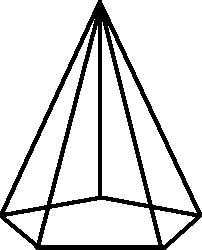
\includegraphics[scale=1]{p-pyramid.png}
\caption{Pentagonal Pyramid with six sides}
\label{fig:pent_p}
\end{figure}

\begin{figure}[h]
\center
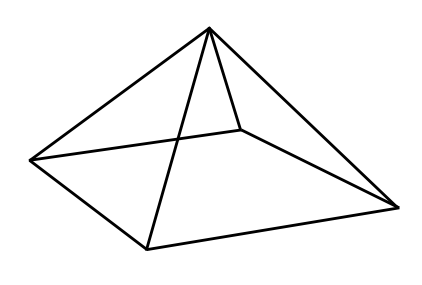
\includegraphics[scale=1]{pyramid_height.png}
\caption{Square Pyramid with five sides}
\label{fig:square_p}
\end{figure}

There were two main reasons for choosing this particular shape:\\
\begin{itemize}
    \item We needed one face with a probability close to half, and the base of a pyramid would be an elegant way to do this.\\
    \item This shape exists for both six and five sided dice, making it easy to extend our simulator and analysis to work for both types.\\
\end{itemize}

\subsection{Optimization Algorithms}
We modelled the pyramidal shape as follows:\\
\begin{itemize}
    \item A height h, denoting the vertical height of the topmost point from the plane containing the base.\\
    \item The origin of our coordinate system is the point vertically below the topmost point lying on the base plane.\\
    \item The first point on the base at a distance $r_1$ from the origin. We define the polar axis to be the line from the origin to this point, so its angle $\theta_1$ is 0.\\
    \item The remaining points on the base, with a distance of $r_i$ and an angle $\theta_i$ from the polar axis, where i goes from 2 to n-1.\\
    \item Note that $\theta_2 < 180$ degrees and $\theta_{n-1} > 180$. This is so that the origin lies within the base. The other values of $\theta_i$ can be any valid angle.\\
\end{itemize}
We now have an object defined by the parameters $h, \theta_i, r_i$ for all i. We also have a cost, the discrepancy, that we have to minimize with certain constraints on the parameters. This looks exactly like an optimization problem, the only difference being that we do not know how exactly the discrepancy varies with each parameter. What we do know, however, is the measured discrepancy over 10000 rolls of the simulator. So we can use certain local search optimization algorithms like simulated annealing or hill climbing. We implemented a hill climbing approach to find a local optimum discrepancy. The neighbours for a particular configuration are formed by changing the height by a small amount, changing the values of $r_i$ and changing $\theta_i$ by small amounts. We formed neighbours and measured the discrepancy of each neighbour. We then chose the neighbour with the lowest discrepancy and repeated the previous step until we reached a local optimum.\\

\subsection{Six Sided Dice}
\subsubsection{Simulator Results}
The optimal parameters found by the simulator after the hill climbing algorithm are:\\
height = 1\\
($r_i$, $\theta_i$) = \\
\{(1, 0)\\
(1.7, 80)\\
(1.2, 144)\\
(0.9, 225)\\
(1.7, 288)\}\\
The angles here are in degrees.\\
Six sided pyramidal die simulation result:\\
calculated probs for side 1: 0.023 (4\%)\\
calculated probs for side 2: 0.0584 (4\%)\\
calculated probs for side 3: 0.2553 (19\%)\\
calculated probs for side 4: 0.0323 (3\%)\\
calculated probs for side 5: 0.1267 (17\%)\\
calculated probs for side 6: 0.5043  (53\%)\\
calculated discrepancy: 0.0115\\

\subsubsection{Improving Accuracy with weights}
The six sided dice had two faces with a very low probability of 4\% on the simulator. Unfortunately, the inconsistencies between the simulator and the physical realization meant that our 3D printed dice could not land on one of the faces. To counter this, we weighted the faulty face by placing a small amount of tape on it, thereby shifting the center of mass closer to this face, allowing the dice to land on it.\\

\subsubsection{Rolling Analysis}


